\documentclass[mat1]{fmfdelo}
% \documentclass[fin1]{fmfdelo}
% \documentclass[isrm1]{fmfdelo}
% \documentclass[mat2]{fmfdelo}
% \documentclass[fin2]{fmfdelo}
% \documentclass[isrm2]{fmfdelo}
\usepackage{tikz}

% naslednje ukaze ustrezno napolnite
\avtor{Nejc Zajc}

\naslov{Enakostranični trikotniki in Jordanove krivulje}
\title{Equilateral triangles and continuous curves}

% navedite ime mentorja s polnim nazivom: doc.~dr.~Ime Priimek,
% izr.~prof.~dr.~Ime Priimek, prof.~dr.~Ime Priimek
% uporabite le tisti ukaz/ukaze, ki je/so za vas ustrezni
\mentor{izred. prof. dr. Aleš Vavpetič}
% \mentorica{}
% \somentor{}
% \somentorica{}
% \mentorja{}{}
% \mentorici{}{}

\letnica{2022} % leto diplome

%  V povzetku na kratko opišite vsebinske rezultate dela. Sem ne sodi razlaga organizacije dela --
%  v katerem poglavju/razdelku je kaj, pač pa le opis vsebine.
\povzetek{Povzetek bo tu}

%  Prevod slovenskega povzetka v angleščino.
\abstract{Abstract goes here}

% navedite vsaj eno klasifikacijsko oznako --
% dostopne so na www.ams.org/mathscinet/msc/msc2020.html
\klasifikacija{}
\kljucnebesede{} % navedite nekaj ključnih pojmov, ki nastopajo v delu
\keywords{} % angleški prevod ključnih besed

\zapisiMetaPodatke  % poskrbi za metapodatke in veljaven PDF/A-1b standard

% aktivirajte pakete, ki jih potrebujete
% \usepackage{tikz}

% za številske množice uporabite naslednje simbole
\newcommand{\R}{\mathbb R}
\newcommand{\N}{\mathbb N}
\newcommand{\Z}{\mathbb Z}
\newcommand{\C}{\mathbb C}
\newcommand{\Q}{\mathbb Q}

% matematične operatorje deklarirajte kot take, da jih bo Latex pravilno stavil
% \DeclareMathOperator{\conv}{conv}

% vstavite svoje definicije ...
%  \newcommand{}{}
\newcommand{\ind}[3][]{\text{ind}_{#1}(#2, #3)}
\newcommand{\arrows}[5][]{
  % arrow with 4 arrow heads
  \draw[->, #1] (#2, #3) -- (0.75*#2 + 0.25*#4, 0.75*#3 + 0.25*#5);
  \draw[->, #1] (0.75*#2 + 0.25*#4, 0.75*#3 + 0.25*#5) -- (0.5*#2 + 0.5*#4, 0.5*#3 + 0.5*#5);
  \draw[->, #1] (0.5*#2 + 0.5*#4, 0.5*#3 + 0.5*#5) -- (0.25*#2 + 0.75*#4, 0.25*#3 + 0.75*#5);
  \draw[->, #1] (0.25*#2 + 0.75*#4, 0.25*#3 + 0.75*#5) -- (#4, #5);
}


\begin{document}

%---------------------------------------------------------------
\section{Uvod}
Že več kot stoletje se matematiki ukvarjajo z na videz preprostim vprašanjem -- ali na vsaki Jordanovi krivulji obstajajo oglišča kvadrata. Ta problem je preprost v formulaciji in hitro razumljiv, a je vseeno do danes ostal nerešen. Prvi ga je leta 1911 postavil nemški matematik Otto Toeplitz \cite{splet_idaho} in v letih, ki so sledila, so matematiki prišli do različnih delnih rezultatov. Podrobno so se raziskala tudi podobna vprašanja, kot na primer iskanje trikotnikov in drugih objektov na Jordanovih krivuljah. V diplomski nalogi si bomo ogledali rezultate pri iskanju trikotnikov in kako smo do njih prišli.

%---------------------------------------------------------------
\section{Osnove}

Za začetek ponovimo in vpeljimo nekatere pojme, ki jih bomo uporabljali pri raziskovanju teme.

\subsection{Terminologija}

Tekom naloge bomo pogosto iskali točke, ki tvorijo oglišča enakostraničnega trikotnika. To lastnost točk $x,\ y$ in $z$ bomo na krajše zapisali kot $xyz \sim \triangle$. Nadalje bomo za točko $x \in X$ rekli da je \emph{ogliščna točka} danega objekta $X$, če obstajata taki točki $y$ in $z \in X$, da $xyz \sim \triangle$.

Ker si bomo natančneje ogledali dogajanje v ravnini, ponovimo definicijo Jordanove krivulje.
\begin{definicija}
\emph{Jordanova krivulja} je sklenjena ravninska krivulja brez samopresečišč. Dobimo jo kot sliko vložitve $f\colon \mathbb{S}^1 \hookrightarrow \R^2$.
\end{definicija}
Glavni izrek glede Jordanovih krivulj je Jordanov izrek.
\begin{izrek}[Jordanov izrek]
Naj bo $J$ Jordanova krivulja v ravnini $\R^2$. Komplement krivulje $\R \setminus J$ sestavljata natanko dve komponenti za povezanost. Ena je omejena in ena neomejena. Krivulja $J$ je meja obeh komponent.
\end{izrek}
Dokaz izreka lahko najdemo v viru \cite{jordan_wiki}. Za Jordanovo krivuljo $J$ v ravnini bomo omejeni komponenti za povezanost $\R \setminus J$ v nalogi rekli \emph{notranjost Jordanove krivulje $J$}. Uporabljali bomo tudi pojem homotopnih preslikav, zato si oglejmo njihovo definicijo.
\begin{definicija}
Naj bosta $X$ in $Y$ podmnožici ravnine in $f,\ g\colon X \to Y$ zvezni funkciji. Homotopija med  $f$ in $g$ je zvezna preslikava
\[
H\colon X \times [0, 1] \to Y,
\]
 za katero velja $H(x, 0) = f(x)$ in $H(x, 1) = g(x)$ za vse $x\in X$.
\end{definicija}
Za homotopijo rečemo, da miruje na robu, če za vsak $t \in [0, 1]$ in za vsako točko $x \in \partial X$ na robu množice $X$ velja $H(x, t) = f(x) = g(x)$.

Definirajmo še strukturo, ki se bo izkazala za zelo pomembno pri obravnavi naše teme.
\begin{definicija}
\emph{Trioda} je poljuben podprostor (v $\R^2$) homeomorfen črki T.
\end{definicija}
Ekvivalentno lahko triodo definiramo kot unijo treh lokov $L_1,\ L_2$ in $L_3$, ki jim pravimo kraki triode, in so paroma disjunktni z izjemo enega skupnega krajišča, v katerem se vsi trije stikajo. Temu krajišču pravimo stičišče krakov. Ostala označimo zaporedoma z $e_1,\ e_2$ in $e_3$ ter jim pravimo končne točke triode.


\subsection{Začetni problem}
Po spoznanih pojmih si oglejmo izrek, ki nam poda odgovor na začetni problem iskanja enakostraničnih trikotnikov na Jordanovi krivulji v ravnini.
\begin{izrek}\label{izr:zacetni}
Vsaka Jordanova krivulja v ravnini vsebuje oglišča enakostraničnega trikotnika.
\end{izrek}
\proof
Naj bo $J$ poljubna Jordanova krivulja v ravnini in $S$ poljubna točka v notranjosti J. Naj bo $C$ krožnica z najmanjšim polmerom s središčem v $S$, ki se dotika $J$. Označimo z $x$ točko v preseku $C \cap J$ ter naj bosta $y_0$ in $z_0$ taki točki na $C$, da $xy_0z_0 \sim \triangle$. Definiramo še spremenljivi točki $y$ in $z$ v ravnini, tako da za $x,\ y$ in $z$ vselej velja $xyz \sim \triangle$. Ko bomo torej premikali eno izmed $y$ ali $z$, se bo premikala tudi druga, tako da se bo ohranjal enakostranični trikotnik $xyz$. Njuni začetni vrednosti definiramo kot $y_0$ in $z_0$.

Sedaj pri fiksnem $x$ začnemo povečevati polmer krožnice $C$ s premikanjem središča vzdolž poltraka $xS$. Tako se $y$ in $z$ oddaljujeta od $x$. Postopek ustavimo, ko $y$ ali $z$ pristaneta na $J$ in na tej točki označimo $y_1 = y$ ter $z_1 = z$. Brez škode za splošnost lahko rečemo $y \in J$. Za konec premaknemo $y$ zvezno do točke $y_2$, ki je točka na $J$, ki je od $x$ najbolj oddaljena. Omenjene točke so označene na naslednji skici.

\begin{center}
\begin{tikzpicture}
\draw [gray] plot [smooth] coordinates {(0,0) (-1.5, 1) (-1.5, -2) (0,-4) (6, -4) (6.5, -2.2) (5, -1.5) (3.464,-2) (2, -1.8) (1, 0.5) (0, 0)};
\filldraw (0,-0.5) circle[radius=1pt];
\draw (0, -0.5) circle (0.5);
\draw[dashed] (0, 0) -- (-0.433 * 3.2, -0.75 * 3.2) -- (0.433 * 3.2, -0.75 * 3.2) -- cycle;
\draw (0,0) -- (-0.433, -0.75) -- (0.433, -0.75) -- cycle;
\node [left] at (-0.433, -0.75) {$y_0$};
\node [right] at (0.433, -0.75) {$z_0$};
\node [left] at (-0.433 * 3.2, -0.75 * 3.2) {$y_1$};
\node [right] at (0.433 * 3.2, -0.75 * 3.2) {$z_1$};

\filldraw (6, -4) circle [radius=1pt];
\node [below] at (6, -4) {$y_2$};

\node [above] at (0, 0) {$x$};

\end{tikzpicture}
\end{center}

Ko se je $y$ premikal od $y_1$ do $y_2$ je tudi $z$ opisal zvezno pot od $z_1$ do $z_2$. Velja, da je $z_1$ ležal na $J$ ali v njegovi notranjosti. Ker sta $y_2$ ter $z_2$ enako oddaljeni od $x$, leži $z_2$ na $J$ ali v neomejeni komponenti $\R^2 \setminus J$. Torej pot, ki jo je opisal $z$, v neki točki seka $J$. Tedaj velja $xyz \sim \triangle$.

\begin{center}
\begin{tikzpicture}
\draw [gray] plot [smooth] coordinates {(0,0) (-1.5, 1) (-1.5, -2) (0,-4) (6, -4) (6.5, -2.2) (5, -1.5) (3.464,-2) (2, -1.8) (1, 0.5) (0, 0)};
\draw (0, 0) -- (0, -4) -- (3.464, -2) -- cycle;
\node [above] at (0, 0) {$x$};

\node [below] at (3.464, -2) {$z$};
\node [below] at (0, -4) {$y$};

\end{tikzpicture}
\end{center}
\endproof

Izrek nam zagotovi obstoj enakostraničnega trikotnika na ravninski Jordanovi krivulji. Koliko takšnih trikotnikov pa lahko najdemo? Naslednja posledica, katere dokaz sledi iz dokaza izreka \ref{izr:zacetni}, nam poda karakterizacijo ogliščnih točk Jordanove krivulje.
\begin{posledica}\label{posl:jordan}
Naj bo $J$ Jordanova krivulja v ravnini in $x \in J$. Točka $x$ je ogliščna točka $J$ natanko tedaj, ko obstajata točki $y$ in $z$, ki ležita na $J$ ali v njegovi notranjosti, tako da velja $xyz \sim \triangle$.
\end{posledica}

Oglejmo si še posledico, ki si natančneje ogleda okolico opazovane točke na $J$.
\begin{posledica}
Naj bo $J$ Jordanova krivulja v ravnini in $x \in J$. Če obstaja tak krog $K$, da leži njegova notranjost $\mathring{K}$ v notranjosti krivulje $J$ in je $K \cap J = \{x\}$, je $x$ ogliščna točka $J$.\\
V posebnem je vsaka točka na gladki Jordanovi krivulji ogliščna.
\end{posledica}
\proof
Ker je $\mathring{K}$ v notranjosti $J$, ležijo vse točke $K$ v notranjosti $J$ ali na $J$. Na krogu $K$ izberemo točki $y$ in $z$, da velja $xyz \sim \triangle$. Ti dve točki izpolnjujeta vse predpostavke posledice \ref{posl:jordan}, zato je točka $x$ ogliščna točka $J$.
\endproof

Preden se konkretneje poglobimo v iskanje enakostraničnih trikotnikov si poglejmo še eno lastnost Jordanovih krivulj v ravnini. Velja namreč, da lahko za poljuben trikotnik v ravnini, na njih najdemo trikotnik, ki mu je podoben.
\begin{trditev}
Naj bosta $T$ poljuben trikotnik in $J$ Jordanova krivulja v ravnini. Tedaj $J$ vsebuje oglišča trikotnika, ki je podoben $T$.
\end{trditev}
\proof
Postopek dokaza je enak postopku dokaza izreka \ref{izr:zacetni}, zato ga še enkrat ponovimo in izpostavimo spremembe. Krožnico $C$ in točko $x$ definiramo kot prej, le da $x$ skupaj s spremenljivima točkama $y$ in $z$ tokrat vselej tvori oglišča trikotnika podobnega $T$. Ta trikotnik naj bo obrnjen tako, da je njegov največji notranji kot pri oglišču $x$. Začetna položaja točk $y$ in $z$ naj bosta točki $y_0$ in $z_0$, ki ležita na $C$. Definirajmo še točki $x_3$ in $y_2$ kot točki na $J$, ki sta najbolj oddaljeni.

Zdaj izvedemo zvezna premikanja točk $y$ in $z$ kot v omenjenem dokazu in na koncu naredimo še naslednji premik. Pri fiksnem $y = y_2$ po krivulji $J$ premaknemo $x$ do $x_3$. Skupna pot točke $z$ je tako sestavljena iz treh zveznih lokov. Ker je $yz$ (ob koncu $y_2z_3$) najdaljša stranica trikotnika, po podobnem premisleku kot prej sledi, da mora $z_3$ ležati na $J$ ali v neomejeni komponenti $\R^2 \setminus J$. Željeni rezultat sledi.
\endproof

V tem razdelku smo videli konstruktivne dokaze za obstoj enakostraničnih trikotnikov na Jordanovih krivuljah. Da se lahko iskanja lotimo bolj sistematično, potrebujemo nekaj novih ravninskih pojmov in objektov.


%--------------------------------------------------------------
\section{Presečno število}\label{razd:presecno}
Glavni nov pojem, ki ga potrebujemo za nadaljne delo, je pojem presečnega števila preslikav. Za dani preslikavi v ravnino, bi radi načrtno prešteli točke preseka njunih slik. S takšnih znanjem bomo kasneje lahko natančno povedali, kje bodo obstajali enakostranični trikotniki.

Naj bo $I = [0, 1] \subset \R$ in naj bosta $f,\ g \colon I \to X \subset \R^2$ taki preslikavi, da zadoščata pogoju
\begin{equation}\label{eq:razl_rob}
\{f(0), f(1)\} \cap g(I) = \emptyset \quad \text{in} \quad \{g(0), g(1)\} \cap f(I) = \emptyset.
\end{equation}
Pojem presečnega števila lahko dobro definiramo le za pare preslikav, ki ustrezajo \eqref{eq:razl_rob}, zato se omejimo na takšne.

Naj bosta za začetek $f$ in $g$ kosoma linearni preslikavi, ki ustrezata \eqref{eq:razl_rob}. Njuni sliki opremimo s standardno usmerjenostjo od slike vrednosti $0$ do slike vrednosti $1$. Ker se poljubni daljici sekata v kvečjemu eni komponenti, velja da je $f(I) \cap g(I)$ zaprta množica, ki vsebuje kvečjemu končno mnogo komponent za povezanost. Te komponente so lahko točke ali kosoma linearne krivulje. Presečno število preslikav bomo definirali kot vsoto presečnih števil komponent preseka njunih slik. V ta namen si najprej oglejmo, kako definiramo presečno število posamezne komponente.

Naj bo $K \subset f(I) \cap g(I)$ komponenta za povezanost, za katero bomo definirali presečno število komponente in ga označili z $\ind[K]{f}{g}$. Najprej denimo, da je $K$ le točka, torej $K = \{x\}$ za nek $x$ v ravnini. V primeru, ko je $x$ točka nelinearnosti $f$ ali $g$ in se sliki preslikav v $x$ ne prečkata, primer tega je prikazan na sliki \ref{fig:presecno_tocka_1}, definiramo $\ind[K]{f}{g} = 0.$ Sicer označimo smerna vektorja slik preslikav $f$ in $g$ v točki $x$ kot $\overrightarrow{s_f}$ in $\overrightarrow{s_g}$, kar prikazuje slika \ref{fig:presecno_tocka_2}. Kot presečno število komponente definiramo
\begin{equation*}
\ind[K]{f}{g} = \begin{cases}
1; & \overrightarrow{s_f}\ \text{in}\ \overrightarrow{s_g}\ \text{tvorita pozitivno orientirano bazo,}\\
-1; &\text{sicer}.
\end{cases}
\end{equation*}

\begin{figure}[h!]
\begin{minipage}{0.5\textwidth}
	\centering
	\begin{tikzpicture}
	\draw[->, blue] (-1,2) -- (1, -2) node[anchor=south east, right] {$f$};
	\draw[gray] (-2, -2) -- (0, 0);
	\draw[->, gray] (0,0) -- (-2, 0.5) node[anchor=north west] {$g$};
	\node[right] at (0, 0) {$x_0$};
	\draw (0, 2.45);
	\end{tikzpicture}
	\caption{$\ind[\{x_0\}]{f}{g} = 0$}
	\label{fig:presecno_tocka_1}
\end{minipage}\hfill
\begin{minipage}{0.5\textwidth}
	\centering
	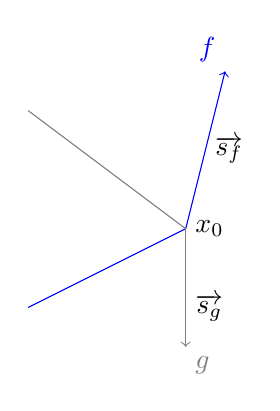
\begin{tikzpicture}
	\draw[blue] (-2, -1) -- (0, 0);
	\draw[->, blue] (0, 0) -- (0.5, 2) node[anchor=south east] {$f$};
	\draw[gray] (-2, 1.5) -- (0, 0);
	\draw[->, gray] (0,0) -- (0, -1.5) node[anchor=north west] {$g$};
	\node[right] at (0, 0) {$x_0$};
	\node[right] at (0.25, 1) {$\overrightarrow{s_f}$};
	\node[right] at (0, -1) {$\overrightarrow{s_g}$};
	\end{tikzpicture}
	\caption{$\ind[\{x_0\}]{f}{g} = -1$}
	\label{fig:presecno_tocka_2}
\end{minipage}
\end{figure}

Druga možnost je, da velja $K \approx J$ za nek interval $J$. Tedaj velja $K = f([a, b])$, za $a,\ b \in (0, 1),\ a < b.$ Prav tako obstaja tak $\varepsilon > 0$, da sta preseka zaprtih krogel z unijo krivulj $\overline{K(f(a), \varepsilon)} \cap (f(I) \cup g(I))$ in $\overline{K(f(b), \varepsilon)} \cap (f(I) \cup g(I))$ linearni triodi s stičišči krakov v $f(a)$ oz. $f(b).$ Linearna trioda je trioda, ki ima za krake daljice. Za določitev presečnega števila najprej preverimo, ali je prišlo do prečkanja preslikav. Zato zavrtimo daljico $\overline{f(a)f(a+\varepsilon)}$ v pozitivni smeri okrog $f(a)$ in daljico $\overline{f(b)f(b-\varepsilon)}$ v negativni smeri okrog $f(b)$, dokler se ne prilegata sliki $f$ ali $g$. Če se po koncu vrtenja obe zavrteni daljici prilegata sliki iste preslikave, kot na sliki \ref{fig:presecno_daljica_1}, definiramo $\ind[K]{f}{g} = 0.$ Sicer nas zanima še relativna usmerjenost teh odsekov. Označimo končni legi zgornjih daljic z vektorjema $\overrightarrow{a}$ in $\overrightarrow{b}$, kjer za smer vzamemo smer slike $f$ oziroma $g$ na tem intervalu. To smo storili na sliki \ref{fig:presecno_daljica_2}. Zanima nas, ali kažeta vektorja v komponento $K$ ali iz nje. Presečno število komponente definiramo kot $1$, če velja $\overline{a} \subset f(I)$ in sta usmerjenosti $\overrightarrow{a}$ in $\overrightarrow{b}$ glede na $K$ različni ali pa velja $\overline{a} \subset g(I)$ in sta usmerjenosti $\overrightarrow{a}$ in $\overrightarrow{b}$ glede na $K$ enaki. Sicer je presečno število komponente enako $-1$. 

\begin{figure}[h!]
\begin{minipage}{0.45\textwidth}
	\centering
	\begin{tikzpicture}
	\draw[->, blue] (-1, -0.333) -- (0, 0) node[pos = 0, above] {$f$};
	\draw (0, 0) -- (1, 1);
	\draw[->, gray] (0.3, -1) -- (0, 0) node[pos = 0, right] {$g$};
	\node[right] at (0, 0) {$f(a)$};
	\draw[->, dashed] (0.354, 0.354) arc (45: 198.4: 0.5);

	\draw[loosely dotted] (1, 1) -- (2, 1);
	\draw (2, 1) -- (3, 0.5);
	\draw[->, blue] (3, 0.5) -- (4.5, 1) node[pos = 1, above] {$f$};
	\draw[->, gray] (3, 0.5) -- (4, -0.5) node[pos = 1, right] {$g$};
	\node [label={[label distance=-10]260:$f(b)$}] at (3, 0.5) {};
	\draw[->, dashed] (2.553, 0.724) arc (153.4: 18.4: 0.5);
 	\draw (0, 3);
	\draw (0, -1.6);
	\end{tikzpicture}
	\caption{$\ind[K]{f}{g} = 0$}
	\label{fig:presecno_daljica_1}
\end{minipage} \hfill
\begin{minipage}{0.45\textwidth}
	\centering
	\begin{tikzpicture}
	\draw[->, blue] (0, 0) -- (1, -1) node[pos = 1, right] {$f$};
	\node[left] at (0.5, -0.5-0.15) {$\vec{b}$};
	\draw (0, 0) -- (1.5, 1);
	\draw[->, gray] (0, 0) -- (-1, -0.333) node[pos = 1, above] {$g$};
	\node[above] at (0, 0) {$f(b)$};
	\draw[->, dashed] (0.416, 0.277) arc (33.7: -45: 0.5);
	
	\draw[loosely dotted] (1.5, 1) -- (2.5, 1);
	\draw (2.5, 1) -- (4, 1.5);
	\draw[->, blue] (5, 2.5) -- (4, 1.5) node[pos = 0, right] {$f$};
	\draw[->, gray] (4.5, 0.5) -- (4, 1.5) node[pos = 0, right] {$g$};
	\node[right] at (4.25, 1) {$\vec{a}$};
	\node [label={[label distance=-10]120:$f(a)$}] at (4, 1.5) {};
	\draw[->, dashed] (3.526, 1.342) arc (198.4: 296.6: 0.5);
	\end{tikzpicture}
	\caption{$\ind[K] {f}{g} = -1$}
	\label{fig:presecno_daljica_2}
\end{minipage} 
\end{figure}

Tako smo definirali presečno število komponente. Preden nadaljujemo, opazimo še, da lahko v zadnjem primeru, ko je $K \approx J$ in $\ind[K]{f}{g} \neq 0$ presečno število določimo kar z obravnavo usmerjenosti smernih vektorjev pri enem oglišču $K$. Označimo kot zgoraj vektor $\overrightarrow{a}$, a zdaj nadaljujemo z vrtenjem v pozitivni smeri okrog $f(a)$, dokler se daljica spet ne prilega sliki $f$ ali $g$. Dobljeni vektor, ki mu smer kot prej določimo glede na krivuljo, ki se ji prilega, označimo s $\overrightarrow{c}$. Ta primer prikazuje slika \ref{fig:presecno_daljica_3}. Velja, da je $\ind[K]{f}{g}$ enako $1$, če je $\overline{a} \subset f(I)$ in sta usmerjenosti $\overrightarrow{a}$ in $\overrightarrow{c}$ glede na $K$ enaki ali pa je $\overline{a} \subset g(I)$ in sta usmerjenosti $\overrightarrow{a}$ in $\overrightarrow{c}$ glede na $K$ različni.  Sicer je presečno število enako $-1$. 

\begin{figure}[h!]
\centering
\begin{tikzpicture}
\draw[->, blue] (0, 0) -- (1, -1) node[pos = 1, right] {$f$};
\draw (0, 0) -- (1.5, 1);
\draw[->, gray] (0, 0) -- (-1.5, -0.5) node[pos = 1, above] {$g$};

\draw[loosely dotted] (1.5, 1) -- (3.5, 1);
\draw (3.5, 1) -- (5, 1.5);
\draw[->, blue] (6, 2.5) -- (5, 1.5) node[pos = 0, right] {$f$};
\node[above] at (5.5, 2) {$\vec{c}$};
\node[right] at (5.25, 1) {$\vec{a}$};
\draw[->, gray] (5.5, 0.5) -- (5, 1.5) node[pos = 0, right] {$g$};
\draw[->, dashed] (4.526, 1.342) arc (198.4: 296.6: 0.5);
\draw[->, dashed] (5.134, 1.231) arc (-63.4: 45: 0.3);
\node [label={[label distance=-10]120:$f(a)$}] at (5, 1.5) {};

\end{tikzpicture}
\caption{Računanje $\ind[K]{f}{g}$ ob enem oglišču}
\label{fig:presecno_daljica_3}
\end{figure}

Kot presečno število kosoma linearnih preslikav lahko zdaj definiramo 
\[
\ind{f}{g} = \sum_{K\ \text{komponenta}} \ind[K]{f}{g}.
\]

Poglejmo si naslednjo lemo, ki bo omogočala lažjo obravnavo presečnega števila.
\begin{lema}\label{le:trikotnik}
Naj bosta $f$ in $\widetilde{f}$ kosoma linearni preslikavi in naj se razlikujeta le na intervalu $(a, b)$, kjer sta $a,\ b \in (0, 1),\ a<b$. Na tem intervalu naj bo $f$ linearna, sliko $\widetilde{f}$ pa naj sestavljata le dve daljici. Če leži trikotnik med omenjenimi daljicami v celoti znotraj $X \setminus \{g(0), g(1)\},$ je $\ind{f}{g} = \ind{\widetilde{f}}{g}$. 
\end{lema}

\begin{figure}[h!]
\centering
\begin{tikzpicture}
\draw[->] (-2, -1) -- (0, 0) -- (3, 0) -- (5, 2) node[pos = 1, above] {$f$}; 
\draw[->] (0, 0) -- (1.5, 2.598);
\node at (1.5, 1.5) {$T$};
\draw[->] (1.5, 2.598) -- (3, 0) node[pos = 0.1, right] {$\widetilde{f}$};
\node[below] at (0, 0) {$f(a)$};
\node[below] at (3, 0) {$f(b)$};
\end{tikzpicture}
\caption{Skica leme \ref{le:trikotnik}}
\end{figure}

\proof
Označimo omenjeni trikotnik s $T$. Dovolj je gledati preseke slik $f,\ \widetilde{f}$ in $g$ na območju T, saj se drugje $f$ in $\widetilde{f}$ ujemata. Ker je tudi $g$ kosoma linearna, si najprej pogledamo kako lahko usmerjena daljica $D$, ki seka $T$, vpliva na presečni števili. Kot prikazuje spodnja slika sta možnosti naslednji.

Lahko sta začetna in končna točka $D$ zunaj $T$. Tedaj $D$ bodisi seka dvakrat sliko $\widetilde{f}$ in nikoli slike $f$ bodisi vsako po enkrat. A ker ima daljica $D$ konstantno smer, prav tako pa sta sliki $f$ in $\widetilde{f}$ enako usmerjeni, se v prvem primeru spremembi presečnega števila $\widetilde{f}$ in $g$ izničita, v drugem pa sta spremembi obeh presečnih števil enaki ($+1$ ali $-1$).

Druga možnost je, da daljica $D$ začne zunaj $T$, konča pa znotraj. Tedaj mora po predpostavki obstajati neka druga daljica, skozi katero slika $g$ zapusti $T$, in vpliv tega primera na presečni števili je enak kot prej. Spremembi obeh presečnih števil sta zopet enaki.


\begin{center}
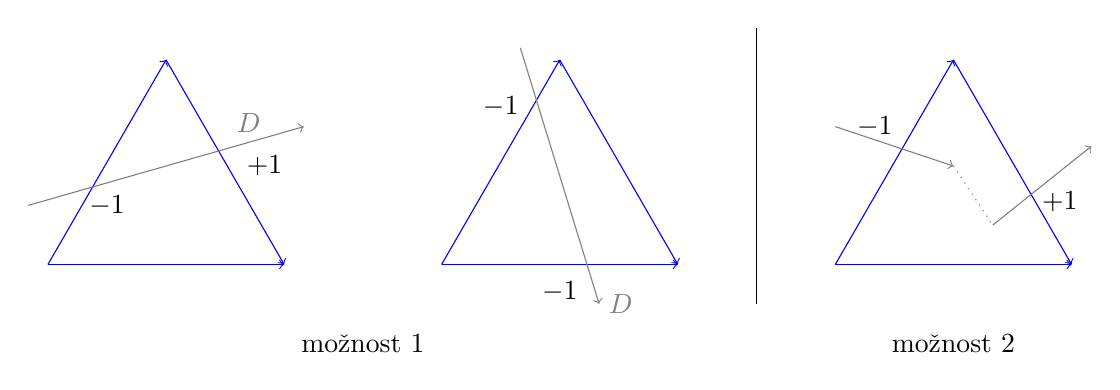
\begin{tikzpicture}
\draw[blue, ->] (0, 0) -- (1.5, 2.598);
\draw[blue, ->] (1.5, 2.598) -- (3, 0);
\draw[blue, ->] (0, 0) -- (3, 0);

\draw[gray, ->] (-0.25, 0.75) -- (3.25, 1.75) node[pos = 0.8, above] {$D$};
\node at (0.75, 0.75) {$-1$};
\node at (2.75, 1.25) {$+1$};

\draw[blue, ->] (5, 0) -- (6.5, 2.598);
\draw[blue, ->] (6.5, 2.598) -- (8, 0);
\draw[blue, ->] (5, 0) -- (8, 0);

\draw[gray, ->] (6, 2.75) -- (7, -0.5) node[pos = 1, right] {$D$};
\node at (5.75, 2) {$-1$};
\node at (6.5, -0.35) {$-1$};

\draw (9, -0.5) -- (9, 3);

\draw[blue, ->] (10, 0) -- (11.5, 2.598);
\draw[blue, ->] (11.5, 2.598) -- (13, 0);
\draw[blue, ->] (10, 0) -- (13, 0);

\draw[gray, ->] (10, 1.75) -- (11.5, 1.25);
\draw[gray, dotted] (11.5, 1.25) -- (12, 0.5);
\draw[gray, ->] (12, 0.5) -- (13.25, 1.5);
\node at (10.5, 1.75) {$-1$};
\node at (12.85, 0.8) {$+1$};

\node at (4, -1) {možnost $1$};
\node at (11.5, -1) {možnost $2$};
\end{tikzpicture}
\end{center}


Ostane obravnavati primer, ko se slika $g$ ujema s katero krivuljo v kosoma linearnem odseku. Če ta odsek ne vključuje niti $f(a)$ niti $f(b)$, je njegov vpliv na presečni števili podoben že obravnavanim primerom in ima tako enaki spremembi za obe. V primeru, da sta tako $f(a)$ kot $f(b)$ del skupnega odseka, sprememb presečnih števil na območju trikotnika $T$ ni in tako trditev leme zopet velja. Zadnja možnost, ko je le ena izmed $f(a)$ in $f(b)$ del skupnega odseka, potrebuje nadaljno ločitev primerov. Ti primeri so podobni že opisanim in vsi vodijo do željene trditve, da sta spremembi obeh presečnih števil na območju trikotnika $T$ enaki.
\endproof

S pomočjo leme \ref{le:trikotnik} lahko dokažemo naslednjo ključno trditev glede dobre definiranosti presečnega števila.
\begin{trditev}
Če obstaja kosoma linearna homotopija $H\colon I \times I \to X \setminus \{g(0), g(1)\}$ med kosoma linearnima preslikavama $f$ in $\widetilde{f}$, ki miruje na robu, je $\ind{f}{g} = \ind{\widetilde{f}}{g}$.
\end{trditev}
\proof
Naj bo $H$ homotopija med kosoma linearnima $f$ in $\widetilde{f}$, za katero veljajo predpostavke trditve. Označimo s $S\subset X$ območje v ravnini, omejeno s krivuljama $f(I)$ in $\widetilde{f}(I)$, za katerega velja $\{g(0), g(1)\} \cap S = \emptyset$. Ker je $H$ kosoma linearna, velja, da lahko $S$ razdelimo na končno število trikotnikov -- med katerimi so lahko nekateri degenerirani -- v katere slika $H$ linearno. 

Definiramo lahko zaporedje preslikav, ki slikajo v $S$, in jih dobimo pri homotopiji med $f$ in $\widetilde{f}$. Začnemo s $f_0 = f$. Nadaljujemo s $f_1$, ki jo dobimo tako, da si izberemo poljuben trikotnik v $S$, ki ima eno izmed stranic na sliki $f_0$ in nato del preslikave $f_0$, ki slika v to stranico, zamenjamo s preslikavo, ki slika isti interval v ostali dve stranici izbranega trikotnika. Tako spremenjeno $f_0$ označimo s $f_1$. Za izbrani trikotnik rečemo, da je že bil uporabljen. Induktivno nato definiramo $f_{k+1}$ iz $f_k$ s spremembo dela preslikave preko enega, še ne uporabljenega trikotnika. Po končnem številu korakov pridemo za nek $N \in \N$ do preslikave $f_N = \widetilde{f}$, kjer postopek ustavimo.

Sedaj uporabimo lemo \ref{le:trikotnik}, ki nam pove, da sta presečni števili $\ind{f_i}{g}$ in $\ind{f_{i-1}}{g}$ enaki za poljuben $i\in \{1, 2, \ldots , N\}$, saj za vse trikotnike $T$ iz $S$ velja $\{g(0), g(1) \} \cap T = \emptyset$. To pomeni, da se presečno število pri prehodih med preslikavami v zaporedju ohranja. Zato velja $\ind{f}{g} = \ind{\widetilde{f}}{g}$.
\endproof

Zdaj lahko sklepamo naslednje. Naj bosta $f$ in $\widetilde{f}$ taki kosoma linearni preslikavi, da med njima obstaja homotopija $H$, ki miruje na robu in slika v $X \setminus \{ g(0), g(1)\}$. Tedaj velja $\ind{f}{g} = \ind{\widetilde{f}}{g}$, saj lahko $H$ po izreku o simplicialni aproksimaciji aproksimiramo s kosoma linearno homotopijo, za katero zdaj vemo, da ohranja presečno število. 

V splošnem lahko torej definiramo presečno število na naslednji način. Naj bosta $f,\ g\colon I \to X$ poljubni ravninski preslikavi, ki ustrezata pogoju \eqref{eq:razl_rob}. Tedaj obstajata $\widetilde{f} \simeq f\colon I \to X \setminus \{g(0), g(1)\}$ in $\widetilde{g} \simeq g\colon I \to X \setminus \{f(0), f(1)\}$ kosoma linearni preslikavi, katerih homotopiji s $f$ in $g$ mirujeta na robu. Njuno presečno število definiramo kot $\ind{f}{g} := \ind{\widetilde{f}}{\widetilde{g}}$. Po vsem prej pokazanem je presečno število dobro definirano, saj se pri prehajanju med homotopnimi kosoma linearnimi preslikavami ohranja.

Tekom naloge bomo presečno število uporabljali tudi na parih usmerjenih krivulj. Za krivulji $A$ in $B$ izberemo regularni parametrizaciji $f_A \colon I \to A$ in $f_B \colon I \to B$, ki slikata vrednost $0$ v začetni točki krivulj. Za presečno število krivulj definiramo $\ind{A}{B} := \ind{f_A}{f_B}$.

\subsection{Rotacija krivulje in presečno število}

Uporabimo zdaj presečno število v okviru tem diplomske naloge. Najprej si poglejmo rotacijo množice okrog neke točke v ravnini.

Za lažji zapis in računanje, si v tem razdelku ravnino predstavljamo kot kompleksno ravnino. Naj bosta $A \subset \C$ in $x \in \C$ poljubna. Definiramo $A_x$ kot rotacijo množice $A$ okrog $x$, natančneje $A_x = \{ y \in \C \mid \exists z \in A: y = k(z-x) + x\}$, kjer je $k = e^{i\pi / 3}$. Primer rotacije prikazuje slika \ref{fig:rotacija_osnovna}. Če je $A$ orientiran lok, $A_x$ orientiramo tako, da je začetna točka loka $A_x$ slika začetne točke loka $A$ pri rotaciji.

\begin{figure}[h!]
\centering
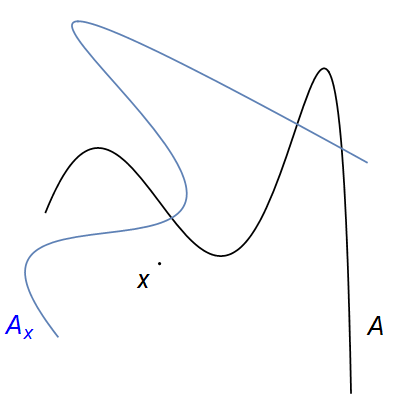
\includegraphics[width = 175pt, height = 175pt]{rotacija_zacetna.png}
\caption{Primer rotacije loka v ravnini}
\label{fig:rotacija_osnovna}
\end{figure}

Naj bo $A$ orientiran lok v kompleksni ravnini $\partial A = \{a_1, a_2\}$ pa njegovi oglišči. Za $x\in \C$ je $\ind{A}{A_x}$ dobro definirano, če je $\partial A \cap A_x = \emptyset = A \cap (\partial A)_x$. Dokažimo še naslednjo lemo, v kateri presečno število $\ind{A}{A_x}$ obravnavamo kot funkcijo točke $x \in \C$ okoli katere zavrtimo $A$, torej $\ind{A}{A_x} \colon \C \to \Z$.

\begin{lema}\label{le:lema2}
\begin{enumerate}
\item Kjer je $\ind{A}{A_x}$ definirano, je zvezno v $x$.
\item Če je $\ind{A}{A_x}$ nedefinirano, potem obstaja tak $y \in A$, da $xya_i \sim \triangle$ za $i \in \{1, 2\}$.
\item Če ne obstajata taka $y$ in $z \in A$, da $xyz \sim \triangle$, sta $A$ in $A_x$ disjunktna in zato je $ind(A, A_x) = 0$.
\item Naj bo $B \subset A$ lok z isto orientacijo kot $A$, za katerega velja $(A \setminus B) \cap A_x = \emptyset$ in $(A_x \setminus B_x) \cap A = \emptyset$. Če sta $\ind{A}{A_x}$ in $\ind{B}{B_x}$ definirana, sta enaka.
\item Če je $S \subset A$ daljica in $x \in S,\ x \notin \partial S$, velja $\ind{S}{S_x} \neq 0$.
\end{enumerate}
\end{lema}

\proof
Vsako točko leme dokažemo posebej, pri dokazu pa bomo uporabili lastnost, da je presečno število dobro definirano preko kosoma linearnih aproksimacij krivulj. Tako lahko dokaz naredimo le za kosoma linearna $A$ in $A_x$.

$(1)$ Zveznost je lokalna lastnost, zato nas zanimajo le možne spremembe pri majhnih spremembah točke $x$. Pokažimo, da se pri takih dogodkih presečno število ne bo spremenilo. Edini položaj krivulj, kjer lahko pri majhnih spremembah točke $x$, kakšna točka preseka izgine ali nastane je, da se krivulji sekata v točki $z_0$ nelinearnosti ene izmed krivulj ter se v tej točki ne prečkata. V tem primeru je $\ind[\{z_0\}]{A}{A_x}=0$. Po tresljaju točke $x$ se lahko zgodi, da v okolici $z_0$ ne bo več nobene točke preseka, kar pomeni, da se presečno število ni spremenilo. Lahko pa v okolici $z_0$ nastane med krivuljama trikotnik. Tako obstajata zdaj dve točki preseka, a ker je relativna smer krivulje, ki predstavlja dve stranici trikotnika, na drugo krivuljo v obeh presečiščih različna, imata presečni števili obeh presečišč različna predznaka. Ko ju seštejemo se torej izničita. Tako smo pokazali, da je pri dovolj majhnih tresljajih točke $x$ presečno število konstantno. Zato je število $\ind{A}{A_x}$ kot funkcija $x$ zvezna.

$(2)$ V primeru, da je presečno število nedefinirano imamo dve možnosti. Za nek $i \in \{1, 2\}$ je lahko: 
\begin{itemize}
\item $a_i = \beta \in A_x$ za nek $\beta \in A_x$. Ker je rotacija $(.)_x$ injektivna, obstaja enoličen $\alpha \in A$, da je $\alpha_x = \beta$. Tedaj velja $a_ix\alpha \sim \triangle$.
\item $(a_i)_x  = \alpha \in A$ za nek $\alpha \in A$. Tudi tokrat velja $a_ix\alpha \sim \triangle$.
\end{itemize}

$(3)$ To točko dokažemo z dokazom obratne implikacije. Denimo, da $A$ in $A_x$ nista disjunktna. Označimo $\alpha \in A \cap A_x$ poljubno točko iz preseka. Tedaj je $\alpha \in A$ in obstaja $\gamma \in A$, da velja $\gamma_x = \alpha$. Pri teh oznakah velja $\alpha x \gamma \sim \triangle$.

$(4)$ Ker je presečno število krivulj $A$ in $A_x$ definirano kot vsota presečnih števil komponent njunega preseka in so vse te vsebovane v $B$, velja $\ind{A}{A_x} = \ind{B}{B_x}$.

$(5)$ Ker je $S$ daljica, se $S$ in $S_x$ sekata le v točki $x$, za katero velja, da ni točka nelinearnosti $S$. Po definiciji za tako komponento preseka velja $\ind[\{x\}]{S}{S_x} \neq 0$. To je tudi edina komponenta preseka, zato je $\ind{S}{S_x} = \ind[\{x\}]{S}{S_x} \neq 0$.
\endproof


%--------------------------------------------------------------
\section{Dognanja v ravnini}
V prejšnjih poglavjih smo spoznali pojme, ki nam bodo sedaj v pomoč pri natančnem odkrivanju dogajanja v ravnini. Izkaže se, da lahko v tem okolju na krivuljah najdemo mnogo trikotnikov. Poglejmo si natančnejše ugotovitve in kako pridemo do njih.
\subsection{Glavni izrek} 
Vemo že, da lahko na poljubni Jordanovi krivulji v ravnini najdemo enakostraničen trikotnik. Prav tako smo spoznali karakterizacijo ogliščnih točk take krivulje. A ne znamo še povedati koliko takšnih točk bo krivulja z gotovostjo imela. Pri odgovoru na to vprašanje bo pomagal naslednji izrek, ki sicer ne govori o Jordanovih krivuljah, ampak o enakostraničnih trikotnikih na ravninskih triodah.
\begin{izrek}\label{izr:glavni}
Trioda $T$  v ravnini vsebuje oglišča enakostraničnega trikotnika, ki ima za eno izmed oglišč končno točko triode $e_1,\ e_2$ ali $e_3$.
\end{izrek}
Triodo $T$ bomo v tem poglavju pogosto omenjali, zato z $L_1,\ L_2$ in $L_3$ označimo še njene krake, s $P$ pa stičišče teh krakov. Pri dokazu izreka si bomo pomagali z dvema lemama. In sicer z lemo \ref{le:lema2}, ki smo jo že spoznali, in z naslednjo lemo.
\begin{lema}\label{le:protislovje}
Predpostavimo, da za triodo $T$ izrek \ref{izr:glavni} ne drži. Tedaj obstaja trioda $T'$ z istimi končnimi točkami $e_1,\ e_2$ in $e_3$, ki vsebuje daljico $S$, za katero velja, da je eno izmed njenih krajišč točka $e_1$. Tedaj ne obstaja niti enakostraničen trikotnik z oglišči na $T'$, ki bi imel za eno izmed oglišč točko $e_1,\ e_2$ ali $e_3$.
\end{lema}

\proof
Zopet si ravnino, ki vsebuje $T$, predstavljajmo kot kompleksno ravnino $\C$. Tako velja $T \times T \subset \C \times \C = \C^2$. Za $j \in \{1, 2, 3\}$ definiramo $E_j$ pomnožice prostora $\C^2$ kot
\[
E_j = \{(w, z) \mid z = e_j + k(w-e_j)\ \text{ali}\ z = e_j + k^{-1}(w-e_j)\},
\]
kjer je $k = e^{i\pi / 3}$. V množicah $E_j$ tako ležijo pari kompleksnih točk, ki s končno točko triode $e_j$ -- znotraj iste kompleksne ravnine -- tvorijo enakostranični trikotnik. Natančneje za točki $a$ in $b$, za kateri $(a, b) \in (T \times T) \cap E_j$, velja $abe_j \sim \triangle$. Predpostavili pa smo, da za $T$ izrek \ref{izr:glavni} ne drži. Zato v omenjenem preseku leži le par točk, ki je v njem vedno. Torej $(T \times T) \cap E_j = \{(e_j, e_j)\}$.

Množica $L_1 \times T$ je kot kartezični produkt kompaktnih množic tudi sama kompaktna množica. Prav tako je $L_1 \times T \subseteq T \times T$ in zato disjunktna z zaprto množico $E_2 \cup E_3$. Zaradi zaprtosti slednje lahko izberemo tak $\delta > 0$, da iz $d(a, L_1)\leq \delta$ in $d(b, T)\leq \delta$ sledi $(a, b) \notin E_2 \cup E_3$. Tu smo z $d(x, M)$ označili razdaljo med točko $x$ in množico $M$ v kompleksni ravnini, ki je za zaprte množice dobro definirana. Po potrebi $\delta$ še nadaljno zmanjšamo, da velja tudi, da iz $e \in T$ in $d(e, e_1) \leq \delta$ sledi $e \in L_1$.

Zdaj imamo definirano vse potrebno za konstrukcijo nove triode $T'$. Začnimo pri stičišču krakov $P$ triode $T$ in potujmo po $L_1$. Označimo s $c$ prvo doseženo točko, za katero je $d(c, e_1) \leq \delta$. Triodo $T'$ definiramo kot $T$, kjer zamenjamo lok med $e_1$ in $c$ z daljico $S$ med omenjenima točkama. Nova trioda $T'$, ki jo vidimo na spodnji sliki, ima končne točke $e_1,\ e_2$ in $e_3$ ter stičišče krakov $P$. Opazimo lahko tudi, da velja $e \in T'$ in $d(e, e_1) = \delta$ natanko tedaj, ko velja $e=c$.

\begin{center}
\begin{tikzpicture}
\draw plot [smooth] coordinates {(0, 0) (1, 1) (3, 0) (4, 2)};
\draw plot [smooth] coordinates {(0, 0) (-1, -1) (-1, -3) (1.5, -4)};
\draw[gray, dashed] plot [smooth] coordinates {(-5, -1) (-4.5, 1) (-3.5, 2) (-3, -0.5) (-2.5, 0)};
\draw plot [smooth] coordinates {(-2.5, 0) (-1, 1) (0, 0)};
\draw (-5, -1) -- (-2.5, 0) node[pos = 0.5, below] {$S$};
\draw[lightgray] (-5, -1) circle (2.693);
\filldraw (0, 0) circle (0.05) node[above] {$P$};
\node[below] at (-5, -1) {$e_1$};
\node[right] at (4, 2) {$e_2$};
\node[right] at (1.5, -4) {$e_3$};
\node at (2, -0.5) {$T'$};
\end{tikzpicture}
\end{center}


Trdimo, da $T'$ ne vsebuje oglišč enakostraničnega trikotnika, ki ima za eno izmed oglišč končno točko $T'$. Dovolj je pokazati, da je $(T' \times T') \cap E_j = \{(e_j, e_j)\}$ za vse $j \in \{1, 2, 3\}$. Naj bo torej $(e, f) \in (T' \times T') \cap E_j$ za nek $j$. Obravnavajmo različne možnosti leg točk $e$ in $f$ ter pri vsaki pokažimo, da se bodisi ne more zgoditi bodisi velja $(e, f) = (e_j, e_j)$.
\begin{enumerate}
\item Naj velja $e,\ f \in T' \setminus S$. Tedaj je $(e, f) \in T \times T$ in zato $(e, f) = (e_j, e_j)$.
\item Naj velja $e \in S$ in $f \in T' \setminus S$. Ker $e$ leži na daljici, je njegova oddaljenost od $L_1$ kvečjemu enaka dolžini daljice. Tako veljata $d(e, L_1)\leq \delta$ in $f \in T$, od tod pa sledi $(e, f) \notin E_2 \cup E_3$. Zato mora veljati $(e, f) \in E_1$. Iz predpisa $E_1$ sledi $d(e, e_1) = d(f, e_1)$. Ampak točka $f$ ne leži na $S$ in zato velja $d(f, e_1) > \delta$, kar je v protislovju z $d(e, e_1) \leq \delta$. Ta primer se torej ne more zgoditi.
\item Tokrat naj velja $f \in S$ in $e \in T' \setminus S$. Zaradi simetrije s prejšnjim primerom lahko sklepamo, da se tudi ta primer ne more zgoditi.
\item Preostane nam obravnavati primer, ko velja $e,\ f \in S$. Tokrat velja $d(e, L_1) \leq d(e, e_1) \leq \delta$ in $d(f, T) \leq d(f, e_1) \leq \delta$, torej zopet sledi da $(e, f) \notin E_2 \cup E_3$. Tako velja $(e, f) \in E_1$. Zaradi predpisa $E_1$ in dejstva da točki $e$ in $f$ ležita na daljici s krajiščem v $e_1$ mora tudi v tem primeru veljati $(e, f) = (e_1, e_1)$.
\end{enumerate}
\endproof

Z ravno dokazano lemo imamo dovolj znanja za naslednji dokaz.

\proof[Dokaz izreka \ref{izr:glavni}]
Izrek bomo dokazali s protislovjem, zato predpostavimo, da na ravninski triodi $T$ ne obstaja enakostranični trikotnik z enim ogliščem v neki izmed končnih točk $e_1,\ e_2$ in $e_3$. Definiramo še $T'$ in $S$ kot v dokazu leme \ref{le:protislovje}. Tokrat z $L_j$ označimo še krake triode $T'$, ki imajo končno točko $e_j$. Definiramo množico $A = L_1 \cup L_2$ in pokažimo protislovje.

\begin{center}
\begin{tikzpicture}
\draw plot [smooth] coordinates {(0, 0) (1.5, -1) (1, -3) (0.5, -4)};
\draw[blue] plot [smooth] coordinates {(-2, 1) (-1, 1.5) (0, 0) (2, 1.5) (5, 0)};
\draw[thick, blue] (-4, 0.5) -- (-2, 1) node[pos = 0.5, below] {$S$};
\node[blue] at (1, 1.5) {$A$};
\filldraw (0, 0) circle (0.05) node[above] {$P$};
\node[below] at (-4, 0.5) {$e_1$};
\node[right] at (5, 0) {$e_2$};
\node[right] at (0.5, -4) {$e_3$};
\node at (-1.25, 0.75) {$L_1$};
\node at (2, 1) {$L_2$};
\node at (0.75, -1.5) {$L_3$};
\end{tikzpicture}
\end{center}

Po točki $(2)$ leme \ref{le:lema2} velja, da je $\ind{A}{A_x}$ dobro definirano v vseh točkah $T'$ razen v krajiščih $A$, saj tam velja $e_1e_1e_1 \sim \triangle$ in $e_2e_2e_2 \sim \triangle$. Vidimo da je množica dobre definiranosti presečnega števila povezana, zato po točki $(1)$ omenjene leme velja, da je $\ind{A}{A_x} \in \Z$ na njej konstantna. Po točki $(3)$ nato velja $\ind{A}{A_x} = \ind{A}{A_{e_3}} = 0$ za vse $x \in T' \setminus \{e_1, e_2\}$.

Zdaj opazimo, da se množici $A$ in $A_{e_1}$ sekata samo v $e_1$. To pomeni, da sta tako $A\setminus S$ in $A_{e_1}$ kot $A_{e_1}\setminus S_{e_1}$ in $A$ na pozitivni razdalji med sabo. Tako lahko izberemo $x \in S$ dovolj blizu $e_1$, da je $x$ edina točka v preseku $A \cap A_x$ in sta tako $A\setminus S$ in $A_x$ kot $A_x \setminus S_x$ in $A$ disjunktna para množic. Ker pa je $S$ daljica, lahko po točkah $(4)$ in $(5)$ leme \ref{le:lema2} sklepamo, da za tak $x$ velja $\ind{A}{A_x} \neq 0$. S tem protislovjem je dokaz končan.
\endproof

\subsection{Posledice}
V zadnjem razdelku smo pokazali, da so triode pomembne pri iskanju enakostraničnih trikotnikov na objektih v ravnini, saj bo vselej vsaj ena njihova končna točka ogliščna. Poglejmo kako nam ta lastnost pomaga pri iskanju večjega števila ogliščnih točk na ravninskih krivuljah in triodah samih. Za začetek si oglejmo posledico, ki govori o zadnjem primeru.
\begin{posledica}\label{posl:trioda}
Vsaka točka nekega kraka ravninske triode $T$, z izjemo stičišča krakov, je ogliščna točka $T$.
\end{posledica}

\proof
Zopet označimo z $L_1,\ L_2$ in $L_3$ krake triode $T$ in s $P$ presečišče njenih krakov. Denimo, da željena trditev ne velja. Tedaj za vsak $j \in \{1, 2, 3\}$ obstaja $a_j \in L_j \setminus P$, tako da nobena izmed naštetih treh točk ni ogliščna točka triode $T$. Definirajmo s $T' \subset T$ novo triodo s končnimi točkami $a_1,\ a_2$ in $a_3$. Tedaj po izreku \ref{izr:glavni} velja, da je za nek $k \in \{1, 2, 3\}$ točka $a_k$ ogliščna za $T'$. To pa seveda pomeni tudi, da je $a_k$ ogliščna točka triode $T$. Tako smo prišli v protislovje.
\endproof

Dokažimo še posledico, ki služi kot končni odgovor na vprašanje obstoja enakostraničnih trikotnikov na Jordanovih krivuljah v ravnini.
\begin{posledica}
Vse razen kvečjemu dveh točk Jordanove krivulje $J$ v ravnini so ogliščne točke $J$.
\end{posledica}
\proof
Denimo da na $J$ obstajajo točke $e_1,\ e_2$ in $e_3$, ki niso ogliščne točke $J$. Ker je notranjost Jordanove krivulje odprta povezana množica, obstaja trioda $T$ s končnimi točkami $e_1,\ e_2$ in $e_3$, ki leži v uniji $J$ in njene notranosti. Po izreku \ref{izr:glavni} je za nek $k \in \{1, 2, 3\}$ točka $e_k$ ogliščna za $T$. To pomeni da obstajata točki $x$ in $y$ na krivulji $J$ ali v njeni notranjosti, da velja $xye_k \sim \triangle$. To so ravno predpostavke posledice \ref{posl:jordan}, ki nam pove, da je točka $e_k$ ogliščna za $J$.
\endproof

Zapisani posledici povesta, da je ogliščnih točk na ravninskih objektih veliko. Hkrati pa sta njuni spodnji meji točni. Hitro lahko namreč najdemo primera, ki ju dosežeta. Sestavimo linearno triodo iz treh daljic tako, da sta kota med zaporednima krakoma pri stičišču enaka $20^\circ$. Stičišče te triode ni ogliščna točka. Primer pri Jordanovih krivuljah je še preprostejši. Vzamemo lahko kar poljuben enakokraki trikotnik, ki ima kot pri vrhu večji od $60^\circ$. V tem primeru oglišči pri osnovnici nista ogliščni točki. Opisana mejna primera prikazuje slika \ref{fig:mejna_primera}.

\begin{figure}[h!]
\centering
\begin{tikzpicture}
\draw (-1*1.5, -2.747*1.5) -- (0, 0) -- (1*1.5, -2.747*1.5);
\draw (0, 0) -- (0, -2.747*1.6);
\draw (0, 0) circle (0.15) node[right] {$P$};


\draw (6, -1) -- (3, -2.5) -- (9, -2.5) -- cycle;
\draw (3, -2.5) circle (0.15) node[below = 4] {$A$};
\draw (9, -2.5) circle (0.15) node[below = 4] {$B$};
\end{tikzpicture}
\caption{Mejna primera triode in krivulje}
\label{fig:mejna_primera}
\end{figure}

%-------------------------------------------------------------
\section{Prostori višjih dimenzij}
Do te točke smo se osredotočali na iskanje trikotnikov v ravnini. Poglejmo si še katere ugotovitve lahko posplošimo na prostore $\R^n$ višjih dimenzij. Pri tem prehodu lahko definicijo ogliščne točke objekta ohranimo enako. Prav tako bomo lastnost treh točk $a,\ b$ in $c \in \R^n$, da tvorijo enakostranični trikotnik še vedno označevali z $abc~\sim~\triangle$. Ravninsko triodo posplošimo povsem naravno samo s spremembo osnovnega prostora v $\R^n$. Tako je trioda še vedno poljuben podprostor homeomorfen črki T. 

Do večjih sprememb pride pri rotaciji krivulje, ki smo jo v ravnini označevali z $A_x$. Ta objekt v več dimenzijah ni več smiseln, zato ga na novo definirajmo. Pri tem se osredotočimo na lastnost, za katero si želimo, da jo množica in njena rotacija imata. Kot v ravnini želimo, da lahko s točkami njunega preseka tvorimo enakostranične trikotnike. Tako je naslednja definicija povsem naravna. Naj bo za $n \geq 2$ množica $A \subset \R^n$. Tedaj za poljuben $x \in \R^n$ definiramo množico rotacije $A$ kot 
\[ A_x = \{y \in \R^n \mid \text{obstaja tak } z \in A, \text{ da velja } xyz \sim \triangle \}. \]

\begin{figure}[h!]
\centering
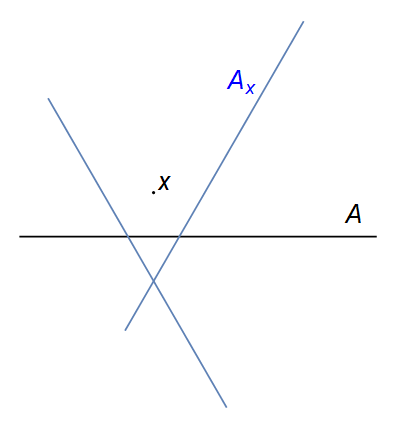
\includegraphics[width = 200pt, height = 200pt]{rotacija_druga_ravnina.png}
\caption{Rotacija daljice v ravnini}
\label{fig:rotacija_sprem_ravnina}
\end{figure}

\begin{figure}[h!]
\centering
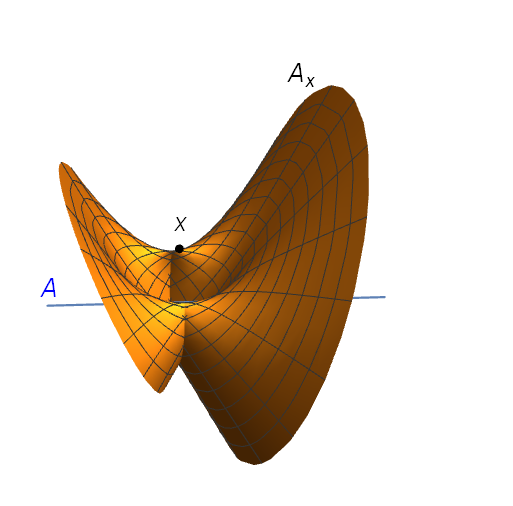
\includegraphics[width = 200pt, height = 200pt]{rotacija_druga_prostor.png}
\caption{Rotacija daljice v prostoru}
\label{fig:rotacija_sprem_prostor}
\end{figure}

Hitro vidimo, da ima definirana rotacija željeno lastnost, a opazimo tudi, da se v ravninskem primeru razlikuje od prejšnje definicije. Zdaj je namreč pri $n=2$ rotacija $A_x$ sestavljena iz 2 krivulj, ki ustrezata rotacijama $A$ v pozitivno in negativno smer. Nadalje v višjih dimenzijah $A_x$ ni več krivulja. Omenjena primera sta predstavljena na slikah \ref{fig:rotacija_sprem_ravnina} in \ref{fig:rotacija_sprem_prostor}, ki prikazujeta rotacijo daljice v ravnini $\R^2$ in prostoru $\R^3$. Pojavi se torej potreba po novi definiciji presečnega števila za krivuljo in ploskev. Poglejmo si pristop v prostoru $\R^3$.

Naj bosta torej zdaj $f \colon I \to X \subset \R^3$ in $g \colon I^2 \to X$. Zanju naj velja, da se ne sekata v robnih točkah poljubne slike, natančneje mora veljati $\{f(0), f(1)\} \cap g(I^2) = \emptyset$ in $\{g(x, y) \mid x \in \{0, 1\} \text{ ali } y \in \{0, 1\} \} \cap f(I) = \emptyset$. To lastnost smo predpostavili, da je presečno število za $f$ in $g$ lahko dobro definirano. Definiramo ga zopet s pomočjo kosoma linearnih aproksimacij, ki obstajajo po izreku o simplicialni aproksimaciji. Naj bosta torej $\widetilde{f} \simeq f \colon I \to X \setminus \{g(x, y) \mid x \in \{0, 1\} \text{ ali } y \in \{0, 1\} \}$ in $\widetilde{g} \simeq g\colon I^2 \to X \setminus \{f(0), f(1)\}$ kosoma linearni preslikavi in naj njuni homotopiji s $f$ in $g$ mirujeta na robu. Presek njunih slik naj bo končen in tako sestavljen iz unije posameznih točk. Če to za neko komponento preseka ne drži, lahko z dovolj malo perturbacijo poljubne preslikave dosežemo, da ostale komponente preseka ostanejo točke, opazovana komponenta pa se v točko spremeni. Naj bo $K = \{x\} \in \widetilde{f}(I) \cap \widetilde{g}(I^2)$ poljubna komponenta preseka. Tedaj obstajajo $a,\ b$ in $c \in I$, da velja $\widetilde{f}(a) = x$ ter $\widetilde{g}(b, c) = x$. Z $\overrightarrow{v}$ označimo smerni vektor standardno usmerjene slike $\widetilde{f}$ v točki $x$, z $\overrightarrow{u_1}$ in $\overrightarrow{u_2}$ pa smerna vektorja koordinatnih krivulj slike $\widetilde{g}$ v točki $x$. Presečno število komponente $K$ defniramo kot
\begin{equation*}
\ind[K]{\widetilde{f}}{\widetilde{g}} = \begin{cases}
1; &\overrightarrow{u_1},\ \overrightarrow{u_2} \text{ in } \overrightarrow{v} \text{ tvorijo pozitivno orientirano bazo prostora,}\\
-1; &\text{sicer}.
\end{cases}
\end{equation*}
S tem lahko definiramo tudi skupno presečno število \[ \ind{\widetilde{f}}{\widetilde{g}} = \sum_{K \text{ komponenta}} \ind[K]{\widetilde{f}}{\widetilde{g}} \] in nato dokončno še \[ \ind{f}{g} := \ind{\widetilde{f}}{\widetilde{g}}. \]

S tem je presečno število za preslikavi $f \colon I \to \R^3$ in $g \colon I^2 \to \R^3$ dobro definirano. V višjih dimenzijah moramo pristopati drugače, a vedno lahko dobro definiramo presečno število za krivuljo in hiperploskev v prostoru $\R^n$. Tako je definicija presečnega števila razširjena na $\R^n$. Lotimo se lahko dokazovanja naslednjega izreka, ki govori o razširjeni lastnosti, ki smo jo v ravnini že dokazali.

\begin{izrek}\label{izr:trioda_prostor}
Ena izmed končnih točk triode $T$ (v prostoru $\R^n$) je ogliščna točka $T$.
\end{izrek} 

Dokazu pristopimo tako kot smo to storili pri dokazu podobnega izreka v ravnini. Z enakimi premisleki, kot v razdelku \ref{razd:presecno}, lahko ugotovimo, da za množico $A \subset \R^3$ še vedno velja lema \ref{le:lema2}. Dokaz leme \ref{le:protislovje} prav tako v višjih dimenzijah še vedno velja. Zamenjati moramo le njegov prvi odstavek. In sicer ga zamenjamo z  naslednjim:

Za $j \in \{1, 2, 3\}$ definiramo množice $E_j \subset \R^{2n}$ kot 
\[
E_j = \{ (w, z) \mid w, z \in \R^n \text{ in } e_jwz \sim \triangle \}.
\] 
Za vse $j$ so $E_j$ zaprte množice. Predpostavka, da izrek \ref{izr:trioda_prostor} ne drži je ekvivalentna pogoju, da za vse $j$ velja $(T \times T) \cap E_j = (e_j, e_j)$.

Dokaz izreka \ref{izr:trioda_prostor} je sedaj enak dokazu izreka \ref{izr:glavni}. Torej lahko tudi v prostoru na triodah najdemo enakostranične trikotnike. Teh je zopet zelo veliko, kot nam pove naslednja posledica z dokazom, ki je enak dokazu posledice \ref{posl:trioda}.

\begin{posledica}
Naj bo $T$ poljubna trioda v prostoru $\R^n$. Tedaj je vsaka točka nekega njenega kraka, z izjemo stičišča krakov, ogliščna točka $T$.
\end{posledica}

Razdelek zaključimo z naslednjo pomembno posledico.

\begin{posledica}
Naj bo $M$ poljubna povezana mnogoterost dimenzije vsaj $2$, ki je vložena v $\R^n$. Tedaj so vse razen kvečjemu dveh točk $M$ ogliščne točke $M$.
\end{posledica}

\proof
Denimo da obstajajo tri točke $e_1,\ e_2$ in $e_3 \in M$, ki niso ogliščne točke $M$. Ker je $M$ povezana in dimenzije vsaj $2$, v $M$ obstaja trioda $T$, ki ima $e_1,\ e_2$ in $e_3$ za končne točke. Tedaj je za nek $k \in \{1, 2, 3\}$ po izreku \ref{izr:trioda_prostor} točka $e_k$ ogliščna točka $T$. A ker je $T \subset M$, to pomeni da je $e_k$ tudi ogliščna točka $M$.
\endproof

%-------------------------------------------------------------
\section{Včrtani štirikotniki}
Oglejmo si nekaj sklepov, do katerih lahko pridemo ob iskanju šritikotnikov na Jordanovih krivuljah v ravnini. Na tem področju so nekatera vprašanja še danes odprta. 

Ne ve se še, ali lahko na poljubni Jordanovi krivulji najdemo oglišča kvadrata. A obstajajo rezultati, do katerih lahko pridemo ob dodatnih omejitvah za krivuljo na kateri iščemo kvadrat. Eden izmed najbolj znanih takšnih rezultatov je naslednji izrek.

\begin{izrek}[Stromquistov izrek]
Če je Jordanova krivulja $J$ ``dovolj lepa'', vsebuje oglišča kvadrata.
\end{izrek}

Izraz ``dovolj lepa'' krivulja $J$ pomeni, da za vsako točko $P$ na $J$ obstaja koordinatni sistem ravnine, v katerem lahko okolico točke $P$ na $J$ dobimo kot graf $y = f(x)$ za zvezno funkcijo $f$. Idejno si lahko rezultat tega izreka predstavljamo kot trditev, da na vsaki Jordanovi krivulji, ki smo jo uspeli s pisalom narisati na papir, obstajajo oglišča kvadrata. Dokaza izreka si ne bomo ogledali, lahko pa ga najdemo v viru \cite{izrek_stromquist}. K iskanju kvadratov na Jordanovih krivuljah lahko pristopimo tudi s pomočjo simetrij, ki nam sicer omejijo možne krivulje, a hkrati zmanjšajo težavnost iskanja kvadratov samih. Oglejmo si naslednji rezultat na to temo.

\begin{trditev}\label{trd:kvadrat}
Vsaka Jordanova krivulja $J$, ki je simetrična glede na izhodišče, vsebuje oglišča kvadrata.
\end{trditev}

\proof
Ker je $J$ simetrična glede na izhodišče koordinatnega sistema, za vsako točko $P \in J$ velja tudi $-P \in J$. Definirajmo si rotacijo $f \colon \R^2 \to \R^2$ za $\frac{\pi}{4}$ okrog izhodišča. Če se $J$ in slika $f(J)$ sekata v točki $P \in J$, potem obstaja $Q \in J$, da $f(Q) = P$. Tedaj so $P,~Q,~-P$ in $-Q$ oglišča kvadrata na $J$.

\begin{center}
\begin{tikzpicture}
\draw plot [smooth cycle] coordinates {(0.5, 0.5) (2, 0) (3, 0.5) (4, -1) (1, -2) (-0.5, -0.5) (-2, 0) (-3, -0.5) (-4, 1) (-1, 2)};
\filldraw (0, 0) circle (0.05) node[below] {$O$};
\node[below] at (-2, 0) {$J$};
\filldraw (0.5, 0.5) circle (0.05) node[right = 3] {$P_b$};
\filldraw (4.05, -0.89) circle (0.05) node[right] {$P_d$};
\draw[dashed] (0.5, 0.5) arc (45: 135: 0.707);
\filldraw (-0.5, 0.5) circle (0.05) node[left] {$f(P_b)$};
\draw[dashed] (4.05, -0.89) arc (-12.4: 77.6: 4.167);
\filldraw (0.89, 4.05) circle (0.05) node[above] {$f(P_d)$};
\end{tikzpicture}
\end{center}


Pokazati ostane, da točka presečišča vselej obstaja. Označimo s $P_b$ in $P_d$ točki na $J$, ki sta zaporedoma najmanj in najbolj oddaljeni od izhodišča. Ker rotacija $f$ ohranja razdaljo točk do izhodišča leži $f(P_b)$ v notranjosti $J$ ali na $J$, točka $f(P_d)$ pa v neomejeni komponenti $\R^2 \setminus J$ ali na $J$, kar je prikazano na zgornji skici. Če katera izmed omenjenih točk leži na $J$, smo našli točko presečišča. V nasprotnem primeru mora slika $f(J)$ povezovati točki na različnih bregovih $J$ in jo tako, zaradi zveznosti $f$, nekje seka.
\endproof

Drugačen način iskanja včrtanih štirikotnikov je s sproščanjem omejitev za iskani lik. Ko ne iščemo več včrtanih kvadratov, pridemo do rezultatov, da na Jordanovi krivulji vselej obstajajo paralelogrami, rombi in pravokotniki. Poglejmo si, kako pokažemo obstoj zadnjih.

\subsection{Včrtani pravokotnik}
Pravokotnik je karakteriziran z naslednjo lastnostjo:
\begin{equation}
\label{prop:pravokotnik}
\text{štirikotnik je pravokotnik} \iff \text{diagonali se razpolavljata in sta enako dolgi}.
\end{equation}
Na ravninski Jordanovi krivulji $J$ tako iščemo dva različna para enako oddaljenih točk, katerih daljici se razpolavljata. Označimo z $X$ množico neurejenih parov različnih točk na $J$.

Postavimo ravnino $\R^2$, ki vsebuje $J$, v prostor $\R^3$ kot ravnino $z = 0$. Definirajmo preslikavo 
\begin{align*}
f &\colon X \to \R^3 \\
f({P, Q}) &= ( \frac{P+Q}{2} , \|P-Q\|).
\end{align*}

\begin{figure}[h!]
\begin{minipage}{0.45\textwidth}
	\centering
	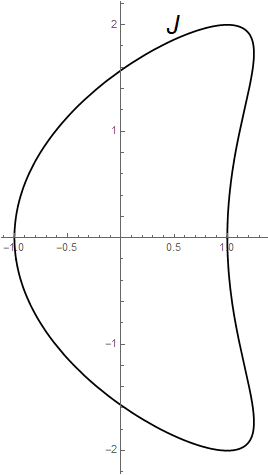
\includegraphics[width = 125pt, height = 175pt]{primer_krivulje.png}
\end{minipage}\hfill
\begin{minipage}{0.45\textwidth}
	\centering
	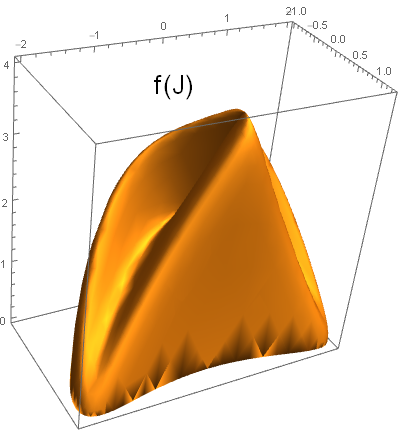
\includegraphics[width = 125pt, height = 175pt]{primer_f_krivulje.png}
\end{minipage}
\caption{Primer Jordanove krivulje in njene slike pri preslikavi $f$}
\end{figure}

Slika te preslikave se dotika krivulje $J$ v ravnini $z=0$. Ko gresta namreč točki v paru $\{P, Q\}$ ena proti drugi, gre razdalja med njima proti nič, prav tako pa gre $(P+Q)/2$ proti isti limitni točki, kot točki sami. Tako gre njuna slika res proti točki na krivulji $J$.
Če uspemo poiskati para $\{P, Q\} \neq \{P,' Q'\}$, ki se s preslikavo $f$ slikata v isto točko, bodo po lastnosti \eqref{prop:pravokotnik} točke teh neurejenih parov sestavljale oglišča pravokotnika na $J$.

Da bomo to lahko storili, si oglejmo, kako lahko predstavimo množico $X$. Jordanova krivulja $J$ je vložitev enotske krožnice $\mathbb{S}^1$ v ravnino. Prav tako je $\mathbb{S}^1$ homeomorfna enotskemu intervalu $I$, ki mu zlepimo začetno in končno točko. Tako lahko točke na $J$ enačimo s števili na $I$. Dve točki na $J$ nam tako predstavlja urejen par $(a, b) \in [0, 1] \times [0, 1]$, kjer enačimo skrajni navpični in vodoravni stranici. Ko v takšnem kvadratu združimo enačene daljice dobimo torus.

A nas zanima množica neurejenih parov točk na $J$, zato moramo enotski kvadrat še spremeniti. Zaradi neurejenosti, sta sedaj para $(P, Q)$ in $(Q, P)$ enaka za poljubna $P,\ Q \in J$. Zato v enotskem kvadratu enačimo vse pare oblike $(a, b)$ in $(b, a)$. Enotski kvadrat smo tako prepognili vzdolž premice $y = x$ in dobili enakokrat trikotnik z enačenima krakoma, kot prikazuje slika \ref{fig:prvi_pregib}. Ker nas zanimajo pari različnih točk, točk na premici $y = x$ ne vključimo v trikotnik, saj predstavljajo posamezne točke na $J$. 

\begin{figure}[h!]
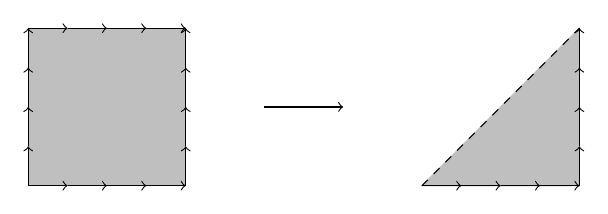
\begin{tikzpicture}
\filldraw[lightgray] (0, 0) -- (2, 0) -- (2, 2) -- (0, 2) -- cycle;
\arrows{0}{0}{2}{0};
\arrows{2}{0}{2}{2};
\arrows{0}{0}{0}{2};
\arrows{0}{2}{2}{2};

\draw[->] (3, 1) -- (4, 1);

\filldraw[lightgray] (5, 0) -- (7, 0) -- (7, 2) -- cycle;
\arrows{5}{0}{7}{0};
\arrows{7}{0}{7}{2};
\draw[dashed] (5, 0) -- (7, 2);
\end{tikzpicture}
\caption{Množica neurejenih parov točk $X$}
\label{fig:prvi_pregib}
\end{figure}

Da najdemo objekt, ki je homeomorfen dobljenemu trikotniku, ga moramo najprej prerezati vzdolž premice $y = 1 - x$. Sedaj lahko zlepimo prvotna kraka trikotnika in dobimo kvadrat, z nasprotno orientiranim parom stranic. Takšen kvadrat je homeomorfen M\"obiusovem traku brez robnih točk, saj tudi kvadrat ni vseboval točk drugega para stranic. Opisani postopek ponazarja zaporedje korakov na sliki \ref{fig:koraki_do_Mob}. Z $M$ označimo M\"obiusov trak in z $g \colon M \to X$ inverz opisane enačitve točk $X$ in $M$. Preslikava $f \circ g$ tako slika M\"obiusov trak v prostor $\R^3$. Sliko M\"obiusovega traku lahko z notranjostjo krivulje $J$ v ravnini $z=0$ dopolnimo do objekta homeomorfnega projektivni ravnini $\R \mathbb{P} ^2$. Injektivnost preslikave $f$, in s tem tudi $f \circ g$, bi tako pomenila obstoj vložitve $\R\mathbb{P}^2$ v $\R^3$, za kar pa vemo, da ne obstaja.


\begin{figure}[h!]
\hfill
\begin{minipage}[b]{0.7\textwidth}
	\centering
	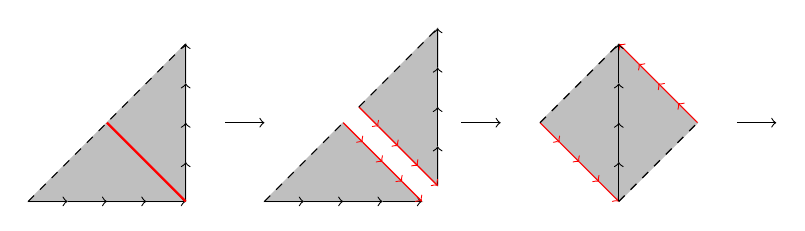
\begin{tikzpicture}
	\filldraw[lightgray] (0, 0) -- (2, 0) -- (2, 2) -- cycle;
	\arrows{0}{0}{2}{0};
	\arrows{2}{0}{2}{2};
	\draw[dashed] (0, 0) -- (2, 2);
	\draw[thick, red] (1, 1) -- (2, 0);
	
	\draw[->] (2.5, 1) -- (3, 1);
	
	\filldraw[lightgray] (3, 0) -- (5, 0) -- (4, 1) -- cycle;
	\arrows{3}{0}{5}{0};
	\arrows[red]{4}{1}{5}{0};
	\draw[dashed] (3, 0) -- (4, 1);
	
	\filldraw[lightgray] (4.2, 1.2) -- (5.2, 0.2) -- (5.2, 2.2) -- cycle;
	\arrows{5.2}{0.2}{5.2}{2.2};
	\arrows[red]{4.2}{1.2}{5.2}{0.2};
	\draw[dashed] (4.2, 1.2) -- (5.2, 2.2);
	
	\draw[->] (5.5, 1) -- (6, 1);
	
	\filldraw[lightgray] (6.5, 1) -- (7.5, 0) -- (8.5, 1) -- (7.5, 2) -- cycle;
	\arrows[red]{6.5}{1}{7.5}{0};
	\arrows[red]{8.5}{1}{7.5}{2};
	\arrows{7.5}{0}{7.5}{2};
	\draw[dashed] (6.5, 1) -- (7.5, 2);
	\draw[dashed] (7.5, 0) -- (8.5, 1);
	
	\draw[->] (9, 1) -- (9.5, 1);
	\end{tikzpicture}
\end{minipage}
\begin{minipage}[b]{0.25\textwidth}
	\centering
	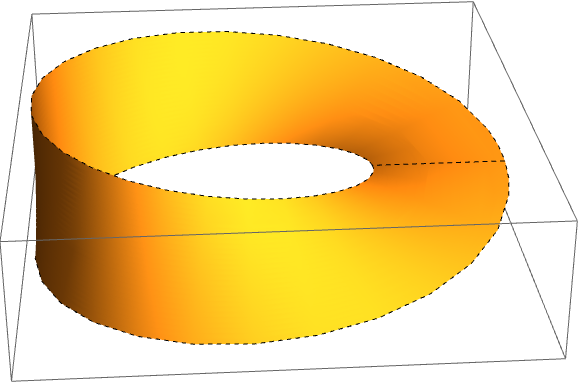
\includegraphics[width = 100pt, height = 70pt]{Mobiusov_trak.png}
\end{minipage}\hfill
\caption{Preoblikovanje predstavitve množice $X$}
\label{fig:koraki_do_Mob}
\end{figure}


Zato obstajata para $\{P, Q\} \neq \{S, T\}$ točk na $J$ z enako sliko. Točke v teh parih so oglišča pravokotnika na $J$.

Opisani postopek je pokazal veljavnost naslednje trditve.
\begin{trditev}
Vsaka Jordanova krivulja $J$ vsebuje oglišča pravokotnika.
\end{trditev}




%------------------------------------------------------------
\section*{Slovar strokovnih izrazov}

\geslo{}{}
\geslo{}{}

% seznam uporabljene literature
\begin{thebibliography}{99}

\bibitem{clanek_meyerson}
M.~D.~Meyerson, \emph{Equilateral triangles and continuous curves}, Fund.\ Math.\ \textbf{110} (1980) 1--9 

\bibitem{izrek_stromquist}
W.~Stromquist, \emph{Inscribed squares and square-like quadrilaterals in closed curves}, Mathematika \textbf{36} (1989) 187--197

\bibitem{splet_idaho}
\emph{Figures Inscribed in Curves}, v: University of Idaho, [ogled 18.~3.~2022], dostopno na \url{https://www.webpages.uidaho.edu/~markn/squares/}.

\bibitem{jordan_wiki}
\emph{Jordan curve theorem}, v: Wikipedia, The Free Encyclopedia, [ogled 18.~3.~2022], dostopno na \url{https://en.wikipedia.org/wiki/Jordan_curve_theorem}.

\end{thebibliography}

\end{document}

